% !TEX root = pfe-book1.tex
%!TEX TS-program = pdflatex
%!TEX encoding = UTF-8 Unicode


\cleardoublepage
\chapter{Motion of Solid Bodies}
\section{Torque}
Try to get a heavy flywheel rotating by hand. Pull
one of the spokes. You will find it difficult if you grasp
it too near to the axle. Move your hand towards the rim,
and thing's will become easier.

But what has chanced? After all, the force is the same
in both cases. The point of application of the force has
changed.

In all that preceded, the question of where a force is
applied did not arise, since the form and size of a body
played no role in the problems under consideration. What
we essentially did was to conceptually replace a body by
a point.

The example with the rotation of a wheel shows that
the question of the point of application of a force is far
from idle when we are dealing with the rotation or revolution of a body.

In order to understand the role of the point of application of a force, let us compute the work which must be
performed to turn a body through a certain angle. In
this calculation, of course, it is assumed that all the particles of the body are rigidly bound to one another (we
are ignoring at present the ability of a body to bend, contract and, in general, to change its form). Therefore, a
force applied to one point of a body imparts kinetic energy to all its parts.

In computing this work, the role of the point of application of a force is clearly seen. A body fastened to an axis is shown in \figr{fig-5-01}. When the body turns through a small angle $\varphi$, the point of application of a force moves along an arc -- it is displaced by a distance $s$.

 \begin{figure}[!ht]
 \centering
 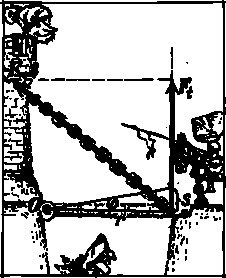
\includegraphics[width=0.45\textwidth]{figures/fig-5-01.pdf}
 \caption{Finding the work done in rotation.}
 \label{fig-5-01}
 \end{figure}

Projecting the force onto the direction of the motion, i.e. onto the tangent to the circle around which the point
of application moves, we find a familiar expression for the work $A$:
 \begin{equation*}%
A  = F_{t} \, s 
 \end{equation*}
But the arc $s$ may be represented as follows:
 \begin{equation*}%
s = r \, \varphi
 \end{equation*}
where $r$ is the distance from the axis of rotation to the
point of application of the force. Thus,
 \begin{equation*}%
A = F_{t} \, r \varphi
 \end{equation*}
Turning the body through one and the same angle in
various ways, we may expend different amounts of work
depending on where the force is applied.

If the angle is given, the work is determined by the
product $F_{t}r$. This product is called the \emph{moment of force}, or the \emph{torque}:
 \begin{equation*}%
M = F_{t} \, r 
 \end{equation*}
Our formula for the torque can be given another form.
Let $O$ be the axis of rotation, and $B$ the point of application of the force \figr{fig-5-02}. The length of the perpendicular dropped from $O$ to the direction of the force is denoted by $d$. The two triangles constructed in the figure are similar. Therefore,
 \begin{equation*}%
\dfrac{F}{F_{t}} = \dfrac{r}{d}  \quad \textrm{or} \quad F_{t} \, r = F \, d
 \end{equation*}
The quantity $d$ is called the \emph{arm}, or the \emph{lever arm}, of the force.

 \begin{figure}[!ht]
 \centering
 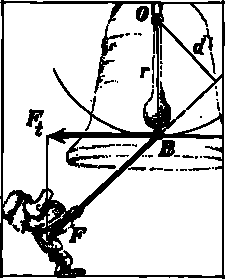
\includegraphics[width=0.45\textwidth]{figures/fig-5-02.pdf}
 \caption{Finding formula for torque.}
 \label{fig-5-02}
 \end{figure}
Our new formula $M = F \, d$ reads as follows: the torque
is equal to the product of the force by its lever arm.

If we displace the point of application of the force along its direction, then the lever arm $d$ and with it the torque
 $M$ will not be changed. Hence, it makes no difference just where the point of application lies on the line of
 action of the force.

With the aid of the new concept, the formula for the
work can be written out more concisely.
\begin{equation*}%
A = M \varphi 
\end{equation*}
i.e. the work is equal to the product of the torque by the angle of rotation.

Let two forces act on a body with moments $M_{1}$ and $M_{2}$.
When the body is rotated through an angle $\varphi$ the work done will be
\begin{equation*}%
M_{1}\varphi + M_{2}\varphi = (M_{1} + M_{2})\, \varphi
\end{equation*}
This equality shows that two forces with moments  $M_{1}$ and $M_{2}$ rotate a body just as a single force with moment $ M = M_{1} + M_{2}$ would. Moments of force can help, as well as hinder, each other. If torques  $M_{1}$ and $M_{2}$ tend to rotate a body in one and the same direction, we should regard them as magnitudes having the same sign. On the contrary, torques rotating a body in opposite directions have different signs.

As we know, the work done by all the forces acting on a body effects a change in its kinetic energy.

The rotation of a body slowed down or speeded up, hence, its kinetic energy changed. This can only take place in case the resultant torque is not equal to zero.

And what if the resultant torque is equal to zero? The answer is obvious -- the kinetic energy does not change; consequently, the body either rotates uniformly by inertia or remains stationary

Thus, the equilibrium of a body capable of rotating requires the balancing of all the torques acting on it. If there are two such torques, the equilibrium requires that
\begin{equation*}%
M_{1} + M_{2} = 0
\end{equation*}
While we were interested in problems in which a body could be regarded as a point, the conditions for equilibrium were simple: in order for a body to remain stationary or move uniformly, stated Newton's law for such problems, it is necessary that the resultant force be equal to zero; the forces acting upwards must balance those directed downwards; the rightward force must compensate for the leftward one.

This law is also valid for our case. If a flywheel is stationary, the forces acting on it are balanced by the reaction of the axle around which the wheel can turn.

But these necessary conditions become insufficient. Besides the balancing of forces, the balancing of torques is also required. The balancing of moments of force is the second necessary condition for the rest or uniform rotation of a solid body.

Torques, if there are several of them, can be easily separated into two groups: some tend to rotate a body clockwise, and others counterclockwise. These are precisely the moments of force which must compensate for each other.

\section{Lever}

Can a person keep 100 tons from falling? Can one crush
a piece of iron with one's hand? Can a child resist a strong
man? Yes, they can.

Ask a strong man to turn a flywheel in the clockwise direction while holding a spoke near the axle. The torque will be small in this case: the force is great but the lever arm is short. If a child pulls the wheel in the opposite direction, holding a spoke near the rim, the torque may turn out to be large: the force is small but the lever arm is long. The condition for equilibrium will be
\begin{equation*}%
M_{1} = M_{2}, \quad \textrm{or} \quad  F_{1}d_{1} = F_{2}d_{2}
\end{equation*}
Using the law of moments, a person can acquire fabulous strength.

The action of levers serves as the most striking example
of this.

You want to lift an enormous stone with the aid of a
crow-bar. This task will turn out to be possible for you
to accomplish, even though the stone weighs several tons.
The crow-bar is placed on a pivot and is the solid body
of our problem. The pivot is the centre of rotation. Two
torques act on the body: a hindering one from the weight
of the stone, and a helping one from your hand. If the
subscript 1 refers to the muscular force, and the subscript
2 to the weight of the stone, the possibility of lifting
the stone can be expressed concisely: $M_{1}$ must be greater than $M_{2}$.

The stone can be supported above the ground provided that
\begin{equation*}%
M_{1} = M_{2}, \quad \textrm{or} \quad  F_{1}d_{1} = F_{2}d_{2}
\end{equation*}

If the short lever arm (from the pivot to the stone) is
fifteen times smaller than the long one (from the pivot
to the hand), then a person acting with his entire weight
on the long end of the lever will support a one-ton stone
in a raised position.

A crow-bar placed on a pivot is a rather widespread and the simplest example of a lever. A ten- to twenty-fold gain in force is usually achieved with the aid of a crow-bar. The length of a crow-bar is about \SI{1.5}{\meter}, but it is usually difficult to place the pivot nearer than \SI{10}{\centi\meter} from its bottom. Therefore, one of the lever arms will be from fifteen to twenty times as long as the other, and so this will also be the gain in force.

A chauffeur will easily raise an automobile weighing several tons with the aid of a jack. A jack is a lever, of the same type as a crow-bar, placed on a pivot. The points of application of the forces (the hand, the weight of the car) lie on opposite sides of pivot of the jack. Here the gain in force is about forty- to fifty-fold, which makes it possible to easily lift an enormous weight.

 \begin{figure}[!ht]
 \centering
 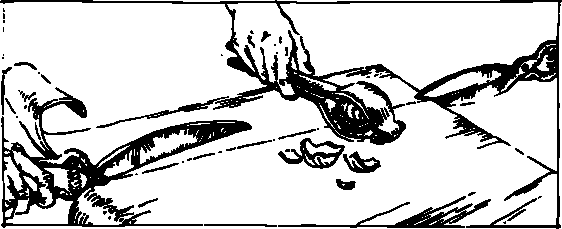
\includegraphics[width=\textwidth]{figures/fig-5-03.pdf}
 \caption{Scissors, nutcracker and plier are all examples of lever.}
 \label{fig-5-03}
 \end{figure}


A pair of scissors, a nutcracker, pliers, pincers, nippers and many other instruments are all levers. You can easily find the centres of rotation (pivots) of the solid bodies depicted in \figr{fig-5-03}, as well as the points of application of the two forces-active and hindering.

In cutting tin-plate with a pair of scissors, one tries to open them as wide as possible. What is accomplished by this? One succeeds in slipping the piece of metal closer to the centre of rotation. The lever arm of the torque one is overcoming becomes shorter, and so the gain in force is greater. When moving a pair of scissors, or nippers, an adult ordinarily acts with a force of 40-50\si{\kilo\gram}\,f. One of the lever arms can be twenty times longer than the other. It turns out that we are able to cut into metal with a force of \SI{1000}{\kilo\gram}\,f. And this with the aid of such simple instruments.

The windlass is a variety of lever. With the aid of a windlass (\figr{fig-5-04}), water is taken out of a well in many villages.

 \begin{figure}[!ht]
 \centering
 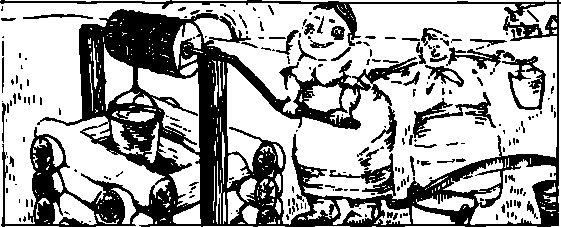
\includegraphics[width=\textwidth]{figures/fig-5-04.pdf}
 \caption{Drawing out water with help of lever, the windlass.}
 \label{fig-5-04}
 \end{figure}

\section{Loss in Path}
Instruments make a person strong, but it by no means
follows from this that instruments permit one to expend
a little work and obtain a lot. The law of conservation of
energy convinces us that a gain in work, i.e, the creation
of work out of ``nothing'', is impossible.

The work obtained cannot be greater than the work
performed. On the contrary, the inevitable energy loss
due to friction leads to the fact that the work obtained
with the aid of an instrument will always be less than that
performed. In the ideal case, these works can be equal.

Properly speaking, we are wasting time by explaining
this obvious truth: for the rule of torques was derived from
the condition of equality of the work performed by the
active and overcome forces.

If the points of application of the forces moved distances
$s_{1}$ and $s_{2}$ the condition of equality of the work assumes
the following form:
\begin{equation*}%
F_{1}^{t}s_{1} = F_{2}^{t}s_{2}
 \end{equation*}
In overcoming some force $F_{2}$ along a path of length $s_{2}$
with the aid of a lever, we can make this by means of
force $F_{1}$ much less than $F_{2}$. But the displacement $s_{1}$ of
our hand must be as many times greater than $s_{2}$ as the muscular force $F_{1}$ is less than $F_{2}$.

This law is often expressed by the following brief sentence: \emph{the gain in force is equal to the loss in path.}

The law of the lever was discovered by the greatest scientist of antiquity -- Archimedes. Amazed at the strength of his proof, this remarkable scientist of antiquity wrote to King Hiero II of Syracuse: ``If there were another world and I could go to it, I would move this one.'' A very long lever whose pivot is near the Earth would make it possible to solve such a problem.

We shall not grieve with Archimedes over the absence of a fulcrum, which, as he thought, was all that he lacked to move the Earth.

Let us dream: take the strongest possible lever, place
it on a pivot and ``suspend a small sphere'' of weight \ldots{} \SI{6e24}{\kgf} on its short end. This modest number shows how much the Earth ``pressed into a small sphere'' weighs. Now apply muscular force to the long end of the lever.

If the force exerted by Archimedes can be taken as
\SI{60}{\kgf}, then in order to displace the ``Earth nut'' by \SI{1}{\centi\meter}, Archimedes' hand would have to cover a distance $\num{6e24})/60 = \num{d23}$ times greater. But \SI{d23}{\centi\meter} are \SI{d18}{\kilo\meter}, which is three billion times greater than the diameter of the Earth's orbit!

This fantastic example clearly demonstrates the scale of the ``loss in path'' involved in the work of a lever.

Any of the examples considered by us above can be used to illustrate not only a gain in force but also a loss
in path. The hand of the chauffeur jacking up his car covers a path which will be as many times longer than the
height to which he raises it as his muscular force is less than the weight of the automobile. Moving a pair of scissors in order to cut a sheet of tin-plate, we perform work along a path which is as many times longer than the depth of the cut as our muscular force is less than the resistance of the tin-plate. The stone lifted by the crow-bar will rise to a height as many times less than that by which the hand is lowered as the muscular force is less than the weight of the stone. This rule clarifies the principle of the
screw's action. Imagine that we are screwing in a bolt, whose threading has a \SI{1}{\milli\meter} screw pitch, with the aid of
a wrench of length \SI{30}{\centi\meter}. The bolt will advance \SI{1}{\milli\meter} along its axis during a single turn, while our hand will cover a \SI{2}{\meter} path during the same time. Our gain in force is two thousand-fold, and we either safely fasten the components together or move a heavy weight with a slight effort of our hand.



\begin{center}
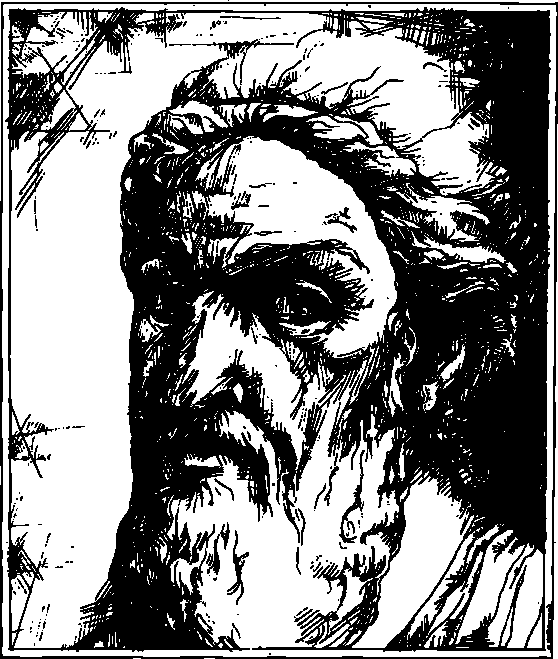
\includegraphics[width=0.8\textwidth]{figures/archimedes.pdf}
\end{center}

{\small \textsf{{Archimedes [c. (287-212) B.C.]}} -- \textsf{\footnotesize The greatest mathematician,
physicist and engineer of antiquity. Archimedes computed the
volume and the surface area of a sphere and its parts, of a
cylinder and of bodies formed by rotating an ellipse, hyperbola
or parabola. He was the first to compute the ratio of the circumference of a circle to its diameter with a high degree of accuracy, showing that it satisfies the inequalities $3 \frac{10}{71} < \pi < 3 \frac{1}{7}$. In mechanics he established the laws of lever, the conditions governing floating bodies (Archimedes' principle), the composition of parallel forces. Archimedes invented the machine for pumping water (Archimedean screw, used in our times for transporting free-flowing or viscous cargo), systems of levers and blocks for raising heavy weights, and military engines successfully employed during the siege of his native city, Syracuse, by the Romans.}}

\section{Other Very Simple Machines}

A loss in path as payment for a gain in force is a general law not only for levers but also for all other devices
and mechanisms used by man.

A tackle is widely used for lifting loads. This is what
we call a system consisting of several movable pulleys
joined to one or several fixed pulleys. The load in \figr{fig-5-05} is suspended by six strings. It is clear that the weight
is distributed among the strings, and so the tension in
a string will be six times less than the weight. The lifting of a one-ton load will require an application of
$1000/6 = \SI{167}{\kgf}$. However, it is not difficult to see that
in order to raise the load by \SI{1}{\meter}, one must haul in \SI{6}{\meter}
of string. For raising the load by \SI{1}{\meter}, \SI{1000}{\kgf\meter} of
work are needed. We must supply this work in ``some form'' -- a force of  \SI{167}{\kgf} must act along a \SI{6}{\meter} path, a force of  \SI{10}{\kgf} along a  \SI{100}{\meter} path, and a force of \SI{167}{\kgf} along a \SI{1}{\kilo\meter} path.
 \begin{figure}[!ht]
 \centering
 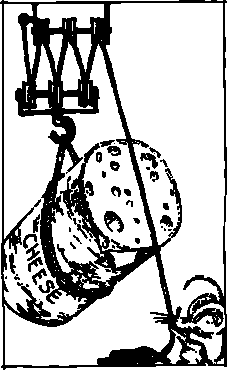
\includegraphics[width=0.45\textwidth]{figures/fig-5-05.pdf}
 \caption{Lifting a heavy weight using a tackle.}
 \label{fig-5-05}
 \end{figure}

An inclined plane, which we discussed on (\pageref{inc-plane}, is also a device permitting a gain in force at the expense of a
loss in path.

A blow is a distinctive means of multiplying forces. A blow with a hammer, an axe, a ram and even a blow with a - fist can create an enormous force. The secret of a strong blow isn't complicated. Driving a nail into an unyielding wall with a hammer, one must take a good wind-up. A big swing, i.e. a long path along which the force acts, generates a significant kinetic energy in the hammer.
This energy is released along a small path. If the swing covers \SI{0,5}{\meter} and the nail enters \SI{0.5}{\centi\meter} into the wall, the force is intensified by a factor of 100. But if the wall is harder and the nail, after the same swing of the hand, enters \SI{0.5}{\milli\meter} into the wall, the blow will be ten times as strong as in the former case. The nail does not enter a hard wall as deeply, and the same work is expended on a shorter path. It turns out that a hammer works like an automaton: it strikes harder where the wall is harder.

If a hammer of \SI{1}{\kilo\gram} is ``speeded up'', it will strike a
nail with a force of \SI{100}{\kgf}. Also, in splitting logs with
a heavy wood-chopper, we break the wood with a force of
several thousands \si{\kgf}'s. Heavy forging hammers fall
from small heights, of the order of a metre. Flattening
a forged piece by \SIrange{1}{2}{\milli\meter}, a hammer of \SI{1000}{\kilo\gram} comes
down on it with an enormous force, that of \SI{d6}{\kgf}.

\section[Adding Parallel Forces Acting on a Solid Body]{How to Add Parallel Forces Acting on a Solid Body}

While solving mechanical problems in which a body
was conceptually replaced by a point, the question of
how to add forces was answered simply on the preceding
pages. The parallelogram law of forces yielded an answer
to this question, and if the forces were parallel, we added
their magnitudes like numbers.

Now matters are more complicated. For the effect of a force on an object is characterized not only by its magnitude and direction but also by the point of its application, or -- we have explained above that this is the same thing -- its line of action.

To add forces means to replace them by a single force. This is by no means always possible.

The replacement of parallel forces by a single resultant
is a problem which can always be solved (except in a
special case, which will be discussed at the end of this
section). Let us consider the addition of parallel forces.
Of course, the sum of forces of \SI{3}{\kgf} and \SI{5}{\kgf} is equal to
\SI{8}{\kgf}, provided that they have the same direction. The
problem consists in finding the point of application (line
of action) of the resultant force.

Two forces acting on a body are depicted in \figr{fig-5-07}.
The resultant force $F$ replaces the forces $F_{1}$ and $F_{2}$, but
this means not only that  $F = F_{1} +F_{2}$; the action of $F$ will be equivalent to that of $F_{1}$ and $F_{2}$ in case the
torque produced by $F$ is equal to the sum of the torques
produced by $F_{1}$ and $F_{2}$.
We are looking for the line of action of the resultant
force $F$. Of course, it is parallel to the forces $F_{1}$ and $F_{2}$,
but how far is this line from $F_{1}$ and $F_{2}$?
 \begin{figure}[!ht]
 \centering
 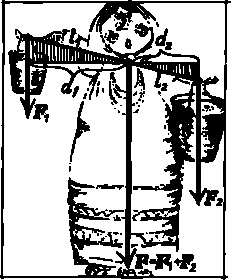
\includegraphics[width=0.45\textwidth]{figures/fig-5-06.pdf}
 \caption{Finding the point of application of the resultant of two parallel forces acting on a body.}
 \label{fig-5-06}
 \end{figure}

A point lying on the segment joining the points of application of $F_{1}$ and $F_{2}$ is depicted in the figure as $F$'s
point of application. With respect to the chosen point, the moment of $F$ is, of course, equal to zero. But then the
sum of the moments of $F_{1}$ and $F_{2}$ with respect to this point should also be equal to zero, i.e. the torques produced by $F_{1}$ and $F_{2}$ opposite in sign will be equal in magnitude.

Denoting the lever arms of $F_{1}$ and $F_{2}$ by $d_{1}$ and $d_{2}$ , we may write out this condition as follows:
\begin{equation*}%
F_{1} d_{1} = F_{2} d_{2} \quad \textrm{or} \quad \dfrac{F_{1}}{F_{2}} = \dfrac{d_{2}}{d_{1}}
\end{equation*}
It follows from the similarity of the shaded triangles that $d_{2}/d_{1} = l_{2}/l_{1}$ i.e. the point of application of the
resultant force divides the distance on the uniting segment between the added forces into parts, $l_{1}$ and $l_{2}$
which are inversely proportional to the forces.

Denote the distance between the points of application
of $F_{1}$ and $F_{2}$ by $l$. It is obvious that $l = l_{1} + l_{2}$.

Let us solve the following system of two equations in two variables
 \begin{align*}%
F_{1} l_{1} - F_{2} l_{2}  & = 0 \\
l_{1} + l_{2} & = l
 \end{align*}
We obtain
\begin{equation*}%
l_{1} = \dfrac{F_{2} l}{F_{1} + F_{2}}, \quad  l_{2} = \dfrac{F_{1}l}{F_{1} + F_{2}}
 \end{equation*}
By means of these formulas, we can find the point of
application of the resultant force not only in the case
when the forces have the same direction but also in the
case of the forces with opposite directions (antiparallel
forces, as we say). If the forces have different directions,
they have opposite signs, and the resultant is equal to the
difference $F_{1} - F_{2}$ of the forces and not to their sum.
Taking the smaller of the two forces, $F_{2}$, to be negative,
we see by our formulas that $l_{2}$ becomes negative. This
means that the point of application of $F_{1}$ lies not to the
left (as before) but to the right of the point of application
of the resultant force \figr{fig-5-07}; moreover, as in the
previous case,
 \begin{equation*}%
\dfrac{F_{1}}{F_{2}} = \dfrac{l_{2}}{l_{1}}
 \end{equation*}
An interesting result is obtained for equal antiparallel forces. Then $F_{1} + F_{2} = 0$. The formulas show that $l_{1}$
and $l_{2}$ will then become infinitely large. What is the physical meaning of this assertion? Since it is meaningless to put the resultant at infinity, it is therefore impossible to replace equal antiparallel forces by a single force.

 \begin{figure}[!ht]
 \centering
 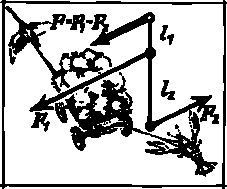
\includegraphics[width=0.45\textwidth]{figures/fig-5-07.pdf}
 \caption{Finding resultant of two anti-parallel forces acting on a body.}
 \label{fig-5-07}
 \end{figure}

Such a combination of forces is called a \emph{couple}.

The action of a couple cannot be reduced to the action
of one force. Any other pair of parallel or antiparallel
forces can be balanced by a single force, but a couple
cannot.

Of course, it would be false to say that the forces constituting a couple cancel each other. A couple has quite a
significant effect -- it rotates a body; the peculiarity of the action of a couple consists in the fact that it does not
produce a translational motion.

In certain cases, the question may arise not of adding
parallel forces but of decomposing a given force into two
parallel ones.
 \begin{figure}[!ht]
 \centering
 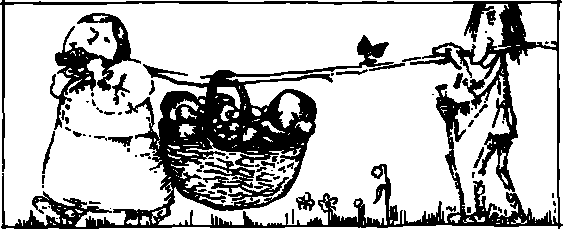
\includegraphics[width=\textwidth]{figures/fig-5-08.pdf}
 \caption{Stronger person should hold the pole nearer to the load.}
 \label{fig-5-08}
 \end{figure}

Two persons carrying a heavy basket together on a
pole are depicted in \figr{fig-5-08}. The weight of the basket
is distributed between the two of them. If the load presses
down on the centre of the pole, they both feel the same
weight. If the distances from the point of application
of the load to the hands which carry it are $d_{1}$ and $d_{2}$, the
force $F$ is decomposed into forces $F_{1}$ and $F_{2}$ according to
the rule
 \begin{equation*}%
 \dfrac{F_{1}}{F_{2}} = \dfrac{d_{2}}{d_{1}}
 \end{equation*}
The stronger person should take hold of the pole nearer
to the load.

\section{Centre of Gravity}

All particles of a body possess weight. Therefore, a solid body is subject to the action of an infinite number of gravitational forces. Moreover, all these forces are parallel. If so, it is possible to add them according to the rules which we have just considered and replace them by a single force. The point of application of the resultant force is called the \emph{centre of gravity}. It is as if the weight
of a body were concentrated at this point.

Let us suspend a body by one of its points. How will it then be situated? Since we may conceptually replace the body by one load concentrated at the centre of gravity, it is clear that in equilibrium this load will lie on the vertical passing through the pivot. In other words, in equilibrium the centre of gravity lies on the vertical passing through the pivot, and is at its lowest possible position.


One can place the centre of gravity on the vertical passing through the axis and above the pivot. It will be very difficult to do this and only because of the presence of friction. Such an equilibrium is unstable. We have already discussed the condition for stable equilibrium -- the potential energy must be minimum. This is precisely the case when the centre of gravity lies below the pivot. Any deflection raises the centre of gravity and, therefore, increases the potential energy. On the contrary, when the centre of gravity lies above the pivot, any puff removing the body from this position leads to a decrease in potential energy. Such a position is \emph{unstable}.

Cut a figure out of cardboard. In order to find its centre of gravity, hang it up twice, attaching the suspending thread first to one and then to another point of the body. Attach the figure to an axis passing through its centre of gravity. Turn the figure to one position, a second, a third, \ldots{} We observe the complete neutrality of the body towards our operations. A special case of equilibrium is attained in any position. This is just what we call it -- \emph{neutral}.

The reason for this is clear -- in any position of the figure, the material point replacing it is located at one and the same place.

In a number of cases, the centre of gravity can be found without any experiments or computations. It is clear, for example, that the centres of gravity of a sphere, circle, square and rectangle are located at the centres of these figures, since they are symmetrical. If we conceptually break up a symmetrical body into small parts, each of them will correspond to another located symmetrically on the other side of the centre. And for each pair of such particles, the centre of the figure will be the centre of gravity.

The centre of gravity of a triangle lies at the intersection of its medians. In fact, let us break up a triangle into narrow strips parallel to one of the sides. A median divides each of the strips in half. But the centre of gravity of a strip lies, of course, half-way along it, i.e. on the median. The centres of gravity of all the strips occur on the median, and when we add their weights, we arrive at the
conclusion that the centre of gravity of the triangle lies somewhere on the median. But this argument is valid with respect to any of the medians. Therefore, the centre of gravity must lie at their intersection.

But perhaps you are not convinced that the three medians intersect in a single point. This is proved in geometry; but our argument also proves this interesting theorem. For a body cannot have several centres of gravity; but since the centre of gravity is one and lies on a median, no matter from which vertex we draw it, all the three medians therefore intersect in a single point. The
formulation of a physical problem helped us prove a geometric theorem.

It is more difficult to find the centre of gravity of a homogeneous cone. It is only clear from considerations of symmetry that the centre of gravity lies on the axis. Computations show that it is located at the distance of a quarter of the height from the base.

The centre of gravity is not necessarily located inside a body. For example, the centre of gravity of a ring is located at its centre, i.e. outside the ring.

Can a pin be placed in a vertical position on a glass pedestal and stay stable?
 \begin{figure}[!ht]
 \centering
 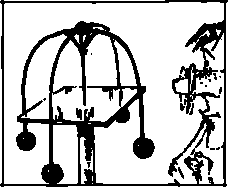
\includegraphics[width=0.6\textwidth]{figures/fig-5-09.pdf}
 \caption{Making a pin stand vertically and stably on a table.}
 \label{fig-5-09}
 \end{figure}
It is shown in \figr{fig-5-09} how to do this. A small apparatus consisting of wires in the form of a double yoke with four small loads should be rigidly fastened to the pin. Since the loads are hanging lower down than the pivot, and the weight of the pin is small, the centre of gravity lies below the pivot. The position is stable.

So far we have been dealing with bodies possessing a point of support. What is the situation in those cases when a body is supported over an entire area element?

It is clear that in this case the location of the centre of gravity above the support does not at all imply that the equilibrium is unstable. How else could glasses stand on a table? It is necessary for stability that the line of action of the gravitational force drawn from the centre of gravity pass through the area of support. On the contrary, if the line of action passes outside the area of support, the body will fall.

Stability may differ greatly depending on how high above the support the centre of gravity is. Only a very clumsy person will overturn a glass of teal but a flower vase with a small base can be overturned by a careless touch. What is the point here?
 \begin{figure}[!ht]
 \centering
 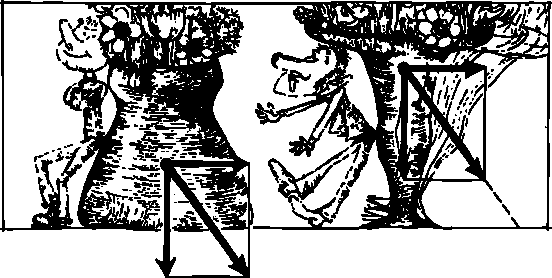
\includegraphics[width=\textwidth]{figures/fig-5-10.pdf}
 \caption{Which vase will tip?}
 \label{fig-5-10}
 \end{figure}
Take a look at \figr{fig-5-10}. Identical horizontal forces are applied to the centres of gravity of two vases. The vase at the right will overturn, since the resultant force doesn't pass through its base but is directed to one side.
 \begin{figure}[!ht]
 \centering
 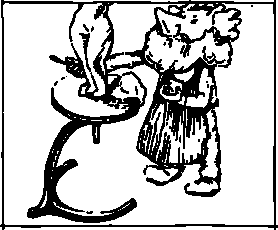
\includegraphics[width=0.6\textwidth]{figures/fig-5-11.pdf}
 \caption{Area of support needed for equilibrium need not be equal to area of actual support.}
 \label{fig-5-11}
 \end{figure}
We have said that for a body to be stable, the force applied to it must pass through the area of support. But the area of support needed for equilibrium does not always correspond to the actual area of support. A body whose area of support has the form of a crescent is depicted in \figr{fig-5-11}. It is easy to see that the stability of the body will not change if the crescent is completed to a solid half-disc. Thus, the area of support determining the condition for equilibrium may be greater than the actual one.

In order to find the area of support for the tripod depicted in \figr{fig-5-12}, one must join its tips with straight-line segments.
 \begin{figure}[!ht]
 \centering
 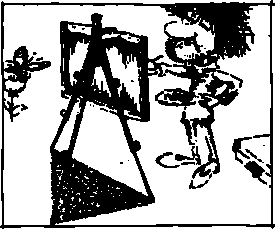
\includegraphics[width=0.6\textwidth]{figures/fig-5-12.pdf}
 \caption{Finding area of support for a tripod.}
 \label{fig-5-12}
 \end{figure}
 
Why is it so hard to walk a tightrope? Because the area of support has sharply decreased. It isn't easy to walk a tightrope, and skilful tightrope walkers aren't rewarded with applause for nothing. However, sometimes viewers make the mistake of acclaiming clever tricks simplifying the task as the epitome of artistry. The performer takes a heavily bent yoke with two pails of water; the pails turn out to be on the level of the tightrope. With a straight face, while the orchestra has ceased playing, the performer takes his walk along the tightrope. How complicated has the trick become, thinks the inexperienced viewer. As a matter of fact, the performer has simplified his task by lowering the centre of gravity.

\section{Centre of Mass}

It is entirely legitimate to ask the following question:
Where is the centre of gravity of a group of bodies? If
many people are on a raft, its stability will depend on
the location of their (together with the raft's) centre of
gravity.

The meaning of this concept remains the same. The
centre of gravity is the point of application of the sum of
the gravitational forces of all the bodies in the group
under consideration.

We know the result of the computation for two bodies.
If two bodies of weights $F_{1}$ and $F_{2}$ are located at a distance
$x$ from each other, their centre of gravity is situated at distances $x_{1}$ from the first body and $x_{2}$ from the second,
where
 \begin{equation*}%
x_{1} + x_{2} = x \quad \textrm{and} \quad \dfrac{F_{1}}{F_{2}} = \dfrac{x_{2}}{x_{1}}
 \end{equation*}
Since weight may be represented as a product $mg$, the centre of gravity of the pair of bodies satisfies the condition
 \begin{equation*}%
m_{1}x_{1} = m_{2}x_{2}
 \end{equation*}
i.e. lies at the point which divides the distance between
the masses into segments inversely proportional to the
masses.

Let us now recall the firing of a gun attached to a platform. The momenta of the gun and the shell are equal in
magnitude and opposite in direction. The following equalities hold:
 \begin{equation*}%
 m_{1} v_{1} = m_{2} v_{2}  \quad \textrm{or} \quad \dfrac{v_{2}}{v_{1}} = \dfrac{m_{1}}{m_{2}} 
 \label{ellipse}
 \end{equation*}
where the ratio of the speeds retains this value during the entire interaction. In the course of the motion arising as a result of the recoil, the gun and the shell are displaced with respect to their initial positions by distances $x_{1}$ and $x_{2}$ in opposite directions. The distances $x_{1}$ and $x_{2}$ -- the paths covered by the two bodies -- increase, but for a constant ratio of speeds, they will also be in the same ratio to each other all the time:
 \begin{equation*}%
\dfrac{x_{2}}{x_{1}} = \dfrac{m_{1}}{m_{2}} \quad \textrm{or} \quad x_{1} m_{1} = x_{2} m_{2}
 \end{equation*}
Here $x_{1}$ and $x_{2}$ are the distances of the gun and the shell from their original positions. Comparing this formula
with the formula determining the position of the centre of gravity, we observe their complete identity. It immediately follows from this that the centre of gravity of the gun and the shell remains at its original position all the time after the firing.

In other words, we have arrived at the very interesting result -- the centre of gravity of the gun and the shell remains stationary after the firing.

Such a conclusion is always true: if the centre of gravity of two bodies was initially stationary, their interaction, regardless of its nature, cannot change the position of the centre of gravity. This is precisely why it is impossible to pick oneself up by the hair or pull oneself up to the Moon by the method of the French writer Cyrano de Bergerac, who proposed (jokingly, of course) to this end that one threw a magnet upwards while holding a piece of iron which would be attracted by the magnet.

A stationary centre of gravity is moving uniformly from the point of view of a different inertial frame of reference. Hence, a centre of gravity is either stationary or moving uniformly and rectilinearly.

What we have said about the centre of gravity of two bodies is also true for a group of many bodies. Of course, for an isolated group of bodies; this is always stipulated when we are applying the law of conservation of momentum.

Consequently, every group of interacting bodies has a point which is stationary or is moving uniformly, and this point is their centre of gravity.

To emphasize the new property of this point, we give it an additional name: the \emph{centre of mass}. As a matter of fact, the question of, say, the weight of the solar system (and hence its centre of gravity) can have only a hypothetical meaning.

No matter how the bodies forming a closed group move, the centre of mass (gravity) will be stationary or, in another frame of reference, will move by inertia.

\section{Angular Momentum}

We shall now become acquainted with another mechanical concept, which permits us to formulate a new important law of motion. This concept is called \emph{angular momentum}, or \emph{moment of momentum}. The very names suggest that we are dealing with the quantity which somehow resembles a moment of force.

A moment of momentum, just as a moment of force, requires the indication of the point with respect to which the moment is defined. In order to define the angular momentum relative to some point, one must construct the momentum vector and drop a perpendicular from the point to its direction. The product of the momentum $m \, v$ by the lever arm $d$ is precisely the angular momentum, which we shall denote by the letter $N$:
 \begin{equation*}%
N = m \, v d
 \end{equation*}
If a body is moving freely, its velocity does not change, the lever arm with respect to any point also remains constant, since the motion takes place along a straight line. Consequently, the angular momentum also remains constant during such a motion.

Just as for the moment of force, we can also obtain a different formula for the moment of momentum. Draw a radius between the position of the body and the point with respect to which we are interested in the angular momentum \figr{fig-5-13}. Construct also the projection of the velocity onto the direction perpendicular to the radius. It follows from the similar triangles constructed in the figure that $v/v_{\perp} = r/d$. Therefore, $vd = v_{\perp}r$, and the formula for angular momentum may also be written in the following form: 
 \begin{equation*}%
N = m \, v_{\perp}r
 \end{equation*}
 \begin{figure}[!ht]
 \centering
 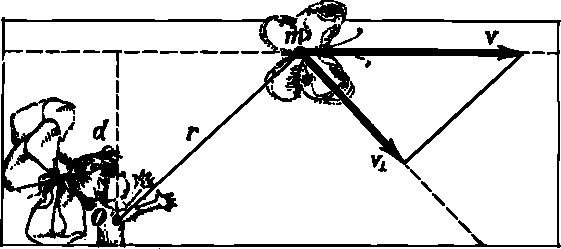
\includegraphics[width=\textwidth]{figures/fig-5-13.pdf}
 \caption{Finding the angular momentum of a body.}
 \label{fig-5-13}
 \end{figure}
 
During free motion, as we have just said, angular momentum remains constant. Well, but if a force is acting on the body? Computations show that the change in angular momentum during a second is equal to the torque. This law can be extended without difficulty to systems of bodies. If we add the changes in the angular momenta of all the bodies belonging to the system in a unit of time, their sum turns out to be equal to the sum of the torques acting on the bodies. Consequently, the following statement is valid for a group of bodies: the change in the total moment of momentum in a unit of time is equal to the sum of the moments of all the forces.

\section{Law of Conservation of Angular Momentum}

If two stones are connected with a string and one of
them is hurled, the other stone will fly after the first at
the end of the stretched string. Each stone will pass the
other, and this forward motion will be accompanied by
a rotation. Let us forget about the gravitational field -- assume that the throw was made in interstellar space.

The forces acting on the stones are equal in magnitude
and directed towards each other along the string (for
these are forces of action and reaction). But then the
lever arms of both forces with respect to an arbitrary point
will also be the same. Equal lever arms and equal but
oppositely directed forces yield torques which are equal
in magnitude and opposite in sign.

The resultant torque will be equal to zero. But it follows from this that the change in angular momentum will
also equal zero, i.e. that the angular momentum of such
a system remains constant.

We only needed the string connecting the stones for visualization. The \emph{law of conservation of angular momentum} is valid for any pair of interacting bodies, no matter what the nature of this interaction.

Yes, and not only for a pair. If a closed system of bodies is being investigated, the forces acting between the bodies can always be divided up into an equal number of forces of action and reaction whose moments will cancel each other in pairs.

The law of conservation of total angular momentum is universal, it is valid for any closed system of bodies.

If a body is rotating about an axis, its angular momentum is
 \begin{equation*}%
N = m \, vr
 \end{equation*}
where $m$ is the mass, $v$ is the speed, and $r$ is the distance from the axis. Expressing the speed in terms of the number $n$ of revolutions per second, we have:
 \begin{equation*}%
v = 2 \pi nr \quad \textrm{and} \quad N = 2 \pi mnr^{2}
 \end{equation*}
i.e. the angular momentum is proportional to the square
of the distance from the axis.

Sit down on a swivel stool. Pick up heavy weights, spread your arms wide apart and ask somebody to get you rotating slowly. Now press your arms to your chest rapidly-you will suddenly begin rotating faster. Arms out-the motion slows down, arms in-the motion speeds up. Until the stool stops turning because of friction, you will have time to change your rotational velocity several times.

Why does this happen?

For a constant number of revolutions per second, the angular momentum would decrease in case the weights approached the axis. In order to ``compensate'' for this decrease, the rotational velocity increases.

Acrobats make good use of the law of conservation of angular momentum. How does an acrobat turn a somersault in mid-air? First of all, by pushing off from an elastic floor or his partner's hand. When pushing off, his body bends forward and his weight, together with the force of the push, creates an instantaneous torque. The force of the push creates a forward motion, and the torque causes a rotation. However, this rotation is slow, incapable of impressing the audience. The acrobat bends his knees. ``Gathering his body'' closer to the axis of rotation, the acrobat greatly increases the rotational velocity and quickly turns over. This is the mechanics of the somersault.

The movements of a ballerina performing a succession of rapid turns are based on this same principle. Ordinarily the initial angular momentum is imparted to the ballerina by her partner. At this instant the dancer's body is bent; a slow rotation begins, then a graceful and rapid movement-the ballerina straightens up. Now all points of her body are closer to the axis of rotation, and conservation of angular momentum leads to a sharp increase in speed.


\section{Angular Momentum as a Vector}
So far we have been dealing with the magnitude of
angular momentum. But angular momentum has the
properties of a vector.

Consider the rotation of a point with respect to some
``centre''. Two nearby positions of the point are depicted
in illustration below \figr{fig-5-14}. The motion in which we are interested is
characterized by the magnitude of its angular momentum
and the plane in which it takes place. The plane of the
motion is shaded in the figure -- it is the area swept out
by the radius drawn from the ``centre'' to the moving
point.
 \begin{figure}[!ht]
 \centering
 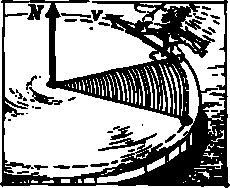
\includegraphics[width=0.65\textwidth]{figures/fig-5-14.pdf}
 \caption{Angular momentum as a vector.}
 \label{fig-5-14}
 \end{figure}
 
Information about the direction of the plane of the
motion and about the magnitude of the angular momentum can be combined. The angular momentum vector,
directed along the normal to the plane of motion and
equal in magnitude to the absolute value of the angular
momentum, serves for this purpose. However, this is
still not all -- one must take into account the direction
of the motion in the plane: for a body can rotate about a
centre in the clockwise as well as in the counterclockwise
direction.

It is customary to draw an angular momentum vector
in such a manner that we see the point rotating in the
counterclockwise direction when we look at it facing the
vector. This can also be said otherwise: the direction of
the angular momentum vector is related to the direction
of the rotation in the same way as the direction of a turning corkscrew is related to the direction of the motion of
its handle.

Thus, if we know the angular momentum vector, we
can determine the magnitude of the angular momentum,
the position of the plane of motion in space, and the direction of the rotation with respect to the ``centre''.

If the motion takes place in one and the same plane,
and the lever arm and speed change, the angular momentum vector preserves its direction in space, but changes
in length. And in the case of an arbitrary motion, the
angular momentum vector changes both in direction and
in magnitude. It may seem that such a fusion into one
concept of the direction of the plane of motion and the
magnitude of an angular momentum serves only the purpose
of saving words. In reality, however, when we are dealing
with a system of bodies moving in more than one plane,
we obtain the law of conservation of angular momentum
only when we add moments of momentum as vectors.
This circumstance shows that the attribution of a vector nature to angular momentum has a profound content.


Angular momentum is always defined with respect to
some conditionally chosen ``centre''. It is only natural that
this quantity depends, generally speaking, on the choice
of this point. Nevertheless, it can be shown that if the
system of bodies under consideration is stationary on the
whole (its total momentum is equal to zero), its angular
momentum vector is independent of our choice of  ``centre''
This angular momentum may be called the internal angular momentum of the system of bodies.

The law of conservation of angular momentum vector
is the third and last conservation law in mechanics. However, we are not being entirely precise when speaking of
three conservation laws. In fact, momentum and angular
momentum are vector quantities, and a law of conservation of a vector quantity implies that not only its magnitude remains constant but also its direction. To put it otherwise, the three components of a vector in three mutually perpendicular directions in space remain constant. Energy is a scalar quantity, momentum is a vector quantity, and angular momentum is also a vector quantity. It would therefore be more precise to say that seven conservation laws hold in mechanics.

\section{Tops}

Try to place a plate topside up on a thin stick and keep
it in a position of equilibrium. Nothing will come of your
efforts. However, this is a favourite trick of Chinese
jugglers. They succeed in performing it with several sticks
simultaneously. A juggler doesn't even attempt to maintain his thin sticks in a vertical position. It appears to
be a miracle that the plates slightly supported by the
ends of the horizontally inclined sticks do not fall and
practically hang in the air.

If you have the opportunity of observing jugglers at
work at close range, note the following significant detail:
the juggler twists the plates in such a fashion that they
rotate rapidly in their planes.

Juggling maces, rings or hats, the performer will in
all cases impart a spin to them. Only then will the objects
return to his hand in the same state in which they were
put at the beginning.

What is the cause of such stability? It is related to
the law of conservation of angular momentum. For when
there is change in the direction of the axis of rotation,
the direction of the angular momentum vector also changes.
Just as a force is needed to change the direction of
velocity, so a torque is needed to change the direction
of rotation; the faster the body rotates, the greater the
torque required.

The tendency of a rapidly rotating body to preserve
the direction of its axis of rotation can be observed in
many cases similar to those mentioned. Thus, a spinning
top does not tip over even if its axis is inclined.

Try to overturn a spinning top with your hand. It
proves to be not so easy to do this.

The stability of a rotating body is utilized in the artillery. You have probably heard that gun barrels are rifled.
An outgoing projectile spins about its axis and, because
of this, does not ``tumble'' through the air. A rifled gun
gives incomparably better aiming and greater range than
an unrifled one.
 \begin{figure}[!ht]
 \centering
 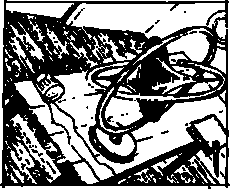
\includegraphics[width=0.65\textwidth]{figures/fig-5-15.pdf}
 \caption{A Cardan suspension (a gyroscope).}
 \label{fig-5-15}
 \end{figure}

It is necessary for a pilot or a sea navigator to always
be aware of the location of the true terrestrial vertical
relative to the position of the airplane or the ship at the
given instant. The use of a plumb-line is unsuitable for
this purpose, since it is deflected during an accelerated
motion. A rapidly spinning top of special construction
is therefore employed-it is called a gyrovertical. If we
set its axis of rotation along a terrestrial vertical, it will
then remain in this position, regardless of how the airplane changes its position in space.

But what does the top stand on? If it is located on a
support which is turning together with the airplane, how
can its axis of rotation preserve its direction?

An apparatus like the Cardan suspension \figr{fig-5-15}
serves as the support. In this apparatus, with a minimum
of friction at the pivots, a top can behave as though it
were suspended in air.

With the aid of spinning tops, it is possible to automatically keep torpedoes and airplanes on a given course.
This is done by means of mechanisms ``watching'' the
deviation of the direction of the torpedo's axis from that
of the top's axis.

Such an important instrument as the gyrocompass is
based on the application of the spinning top. It can be
proved that under the action of the Coriolis force and
friction, the top's axis eventually settles down parallel
to the Earth's axis, and so points to the North.

Gyrocompasses are widely applied in navigation. Their
main part is an engine with a heavy flywheel which does
up to \num{25000}~rpm.

In spite of a number of difficulties involved in the elimination of various hindrances, in particular those due
to the pitching of a ship, gyrocompasses have an advantage over magnetic compasses. The drawback of the latter
is the distortion of the readings because of the influence
of iron objects and electrical appliances aboard the ship.

\section{Flexible Shaft}

Shafts are important parts of modern steam turbines. The manufacture of such shafts which are \SI{10}{\meter} in length and \SI{0.5}{\meter} in diameter is a complex technological problem. The shaft of a powerful turbine can withstand a load of about 200~ton and rotate with a speed of 3000~rpm.

At first glance, it might seem that such a shaft should
be exceptionally hard and durable. This, however, is
not so. At tens of thousands of revolutions per minute,
a rigidly fastened and unbendable shaft will inevitably
break, no matter how strong it may be.

It isn't difficult to see why rigid shafts are unsuitable.
No matter how precisely engineers work, they cannot
avoid at least a slight asymmetry in the wheel of a turbine.
Enormous centrifugal forces arise when such a wheel
rotates; recall that their magnitudes are proportional to
the square of the rotational speed. If they are not exactly
balanced, the shaft will start ``beating'' against the ball
bearings (for the unbalanced centrifugal forces ``rotate''
together with the machine), break them and smash the
turbine.

At one time, this phenomenon created an unsurmountable obstacle to the increase in the rotational speed of
a turbine. A way out of the situation was found at the
last turn of the century. The flexible shaft was introduced
into the technology of turbine construction.

In order to understand the idea behind this remarkable
invention, we must compute the total effect of the centrifugal forces. But how can these forces be added? It turns
out that the resultant of all the centrifugal forces acts
at the centre of gravity of the shaft and has the same magnitude as if the entire mass of the wheel of the turbine were
concentrated at the centre of gravity.

Let us denote the distance from the centre of gravity
of the wheel of the turbine to its axis, distinct from zero
because of a slight asymmetry in the wheel, by $a$. During
rotation, centrifugal forces will act on the shaft which
will bend. Denote the displacement of the shaft by $l$.

Let us compute this magnitude. We know the formula
for centrifugal force (see p.~\pageref{centrifugal}). This force is proportional
to the distance from the centre of gravity to the axis,
which is now $a+l$, and is equal to $4 \pi^{2} n^{2} M (a + l)$,
where $n$ is the number of revolutions per minute, and $M$
is the mass of the rotating parts. The centrifugal force is
balanced by the elastic force, which is proportional to the
magnitude of the displacement of the shaft and is equal
to $kl$, where the coefficient $k$ characterizes the rigidity of
the shaft. Thus:
 \begin{equation*}%
kl= 4 \pi^{2} n^{2} M (a+l)
 \end{equation*}
whence
 \begin{equation*}%
l= \dfrac{a}{k/4 \pi^{2} n^{2} M - 1}
 \end{equation*}
Judging by this formula, fast rotations are no problem
for a flexible shaft, For very large (even infinitely large)
values of $n$, the deflection $l$ of the shaft does not grow
without bound. The value of $k/4 \pi^{2} n^{2} M$ figuring in our
last formula tends to zero, and the deflection $l$ of the shaft
becomes equal in magnitude to the asymmetry, but opposite in sign.

This computational result implies that, for fast rotations, the asymmetrical wheel, instead of smashing the
shaft, bends it in such a way as to cancel the effect of
asymmetry. The bending shaft centres the rotating parts,
transfers the centre of gravity to the axis of rotation by
means of its deformation, and thus nullifies the action of
the centrifugal force.

The flexibility of the shaft is by no means a drawback;
on the contrary, it is a necessary condition for stability.
As a matter of fact, it is necessary for stability that the
shaft bend by a distance of the order of a without breaking.

An attentive reader may have noticed an error in the
reasoning employed. If we displace a shaft ``centring''
during fast rotations from the position of equilibrium we
have found and consider only centrifugal and elastic
forces, it is easy to see that this equilibrium is unstable.
It turns out, however, that Coriolis forces save the situation and make this equilibrium quite stable.

A turbine starts turning slowly. At first, when $n$ is very small, the fraction $k/4\pi^{2}n^{2}M$ will be great. As long as this fraction is greater than unity with increasing $n$, the deflection of the shaft will have the same sign as that of the original displacement of the centre of gravity of the wheel. Therefore, at the beginning of the motion the bending shaft does not centre the wheel, but, on the contrary, increases the total displacement of the centre of gravity by means of its deformation, and hence also the centrifugal force. To the degree that $n$ increases (with the condition $k/4\pi^{2}n^{2}M > 1$ preserved), the displacement grows and, finally, the critical moment is reached. 

The denominator of our formula for the displacement $l$ vanishes when $k/4\pi^{2}n^{2}M = 1$, and so the deflection of the shaft formally becomes infinitely large. The shaft will break at such a speed of rotation. In starting a turbine this moment must be passed very quickly; it is necessary to slip by the critical number of revolutions per minute and pass over to a much faster motion of the turbine for which the phenomenon of self-centring described above will begin.

But what is this critical moment? We can rewrite its condition in the following form:
 \begin{equation*}%
4 \pi^{2} \dfrac{M}{k}   =  \dfrac{M}{n^{2}}
 \end{equation*}
Or, expressing the number of revolutions per minute in terms of the period of rotation by means of the relation $n = 1/ T$ and extracting square roots, we can rewrite it as follows:
 \begin{equation*}%
T  = 2 \pi  \, \sqrt{\dfrac{M}{k}}
 \end{equation*}
But what kind of quantity have we obtained in the right-hand side of the equality? Our formula looks rather familiar. Turning to p.~\pageref{pend-osc}, we see that the period of free vibration of the wheel on the shaft figures in our right-hand side. The period $2 \pi \sqrt{ M/k}$ is that with which the wheel of a turbine of mass $M$ would vibrate on a shaft of rigidity $k$ if we were to deflect the wheel to one side, so that it might vibrate by itself.

Thus, the dangerous instant is when the rotational period of the wheel of the turbine coincides with the period of free vibration of the system turbine-shaft. Resonance is responsible for the existence of a critical number of revolutions per minute.
